\documentclass[12pt,onecolumn,a4paper]{article}
\usepackage{epsfig,graphicx,subfigure,amsthm,amsmath}
\usepackage{color,xcolor}     
\usepackage{xepersian}
\usepackage{cite}
\usepackage{fontspec}
\usepackage{multirow}

\settextfont[Scale=1]{BMitra}
\setlatintextfont[Scale=0.8]{Vazir-Regular}


\begin{document}
\title{گزارش تکلیف ۵ درس یادگیری ماشین} 
\author{کسرا سینایی\\
شماره دانشجویی ۸۱۰۶۹۶۲۵۴\\
}
\date{\today}
\maketitle
\thispagestyle{empty}
\newpage
\section*{سؤال یک}
\subsection*{الف}
روش‌های جست و جو:
\begin{description}
    \item[$\bullet$] \lr{Exhustive}: در این روش‌ها تمام حالات ممکن برای به دست آوردن زیرمموعه‌ای از فیچرها امکان پذیر است در نظر گرفته می‌شوند. اگر $n$ فیچر داشته باشیم، پیچیدگی محاسباتی این روش $O(n^{2})$ است. به دلیل پیچیدگی محاسباتی بالا، این روش معمولا کاربردهای کمی دارند (مثال: \lr{Breadth First Search})
    \item[$\bullet$] \lr{Heuristic}: روش‌هایی مانند \lr{SFS}، \lr{SBS}، \lr{BDS}  و ... هستند. در این روش‌ها یا با مجموعه‌ی کامل فیچرها شروع کرده و به ترتیب فیچرهایی که حذف آن‌ها بهینه ترین زیرمجموعه جدید را نتیجه دهد حذف می‌شوند، یا با زیرمجوعه تهی از فیچرها شروع کرده و به مرور فیچرهایی را که بهینه ترین زیرمجموعه جدید را حاصل می‌کنند اضافه می‌شوند به زیرمجموعه فیچرها.
    \item[$\bullet$] \lr{Randomize}: در این روش ابتدا به صورت اتفاقی زیرمجموعه‌ای از فیچرها انتخاب می‌شوند، سپس با استفاده از الگوریتم‌هایی مانند ژنتیک، \lr{RGSS} و ... به بهینه سازی تابع هزینه می‌پردازند تا زیرمجموعه بهینه از فیچرها به دست آید.
\end{description}
روش‌های ارزیابی:
\begin{description}
    \item[$\bullet$] \lr{Filter Methods}: این روش‌ها بدون توجه به اللگوریتم طبقه‌بندی زیرمجموعه انتخابی از فیچرها را ارزیابی می‌کنند. معیار اصلی ارزیابی اطلاعات موجود در هر زیرمجموعه از فیچر است. این روش‌ها سریع هستند و تمایل به انتخاب زیر مجموعه‌های بزرگی از فیچرها را داغرند.
    \item[$\bullet$] \lr{Wrpper Methods}: برای ارزیابی زیرمجموعه انتخاب شده از فیچرها، معیارهایی در نظر گرفته می‌شود که به الگوریتم طبقه بندی مربوط است. برای مثال پروسه ارزیابی کیفیت زیرمجموعه فیچر انتخاب شده از دقت آن در پیش بینی تعدادی داده تست استفاده می‌شود. این روش‌ها آهسته هستند اما دقیق تر از \lr{Filter Methods} کار می‌کنند.
\end{description}
\subsection*{ب}
در محاسبات \lr{LDA} لازم است معکوس ماتریس $S_w$ را حساب کرد و سپس مقادیر ویژه و بردارهای ویژه $S_{w}^{-1}S_{b}$ را به دست آورد. با افزایش ابعاد مسئله حجم محاسبات جبری افزایش می‌یابد. همچنین اگر تعداد نمونه‌ها کم باشد ممکن است ماتریس $S_{w}$ سینگولار شود.
\\
در \lr{PCA} نیز باید مقادیر ویژه ماتریس کواریانس نمونه‌ها و بردارهای متناظر با آن‌ها محاسبه شوند تا \lr{PC}ها به دست آیند. اگر ابعاد مسئله زیاد شود علاوه بر حجم محاسباتی مقادیر ویژه امکان کاهش دقت تخمین ماتریس کواریانس هم به وجود می‌آید. یکی از نقاط ضعف \lr{PCA} حساسیت ان به اسکیل فیچرها می‌باشد به همین دلیل نرمال کردن دیتا قبل از اجرای الگوریتم اهمیت ویژه‌ای دارد.
\\

\newpage
\section*{سوال دو}
\begin{figure}[h!]
    \begin{center}
    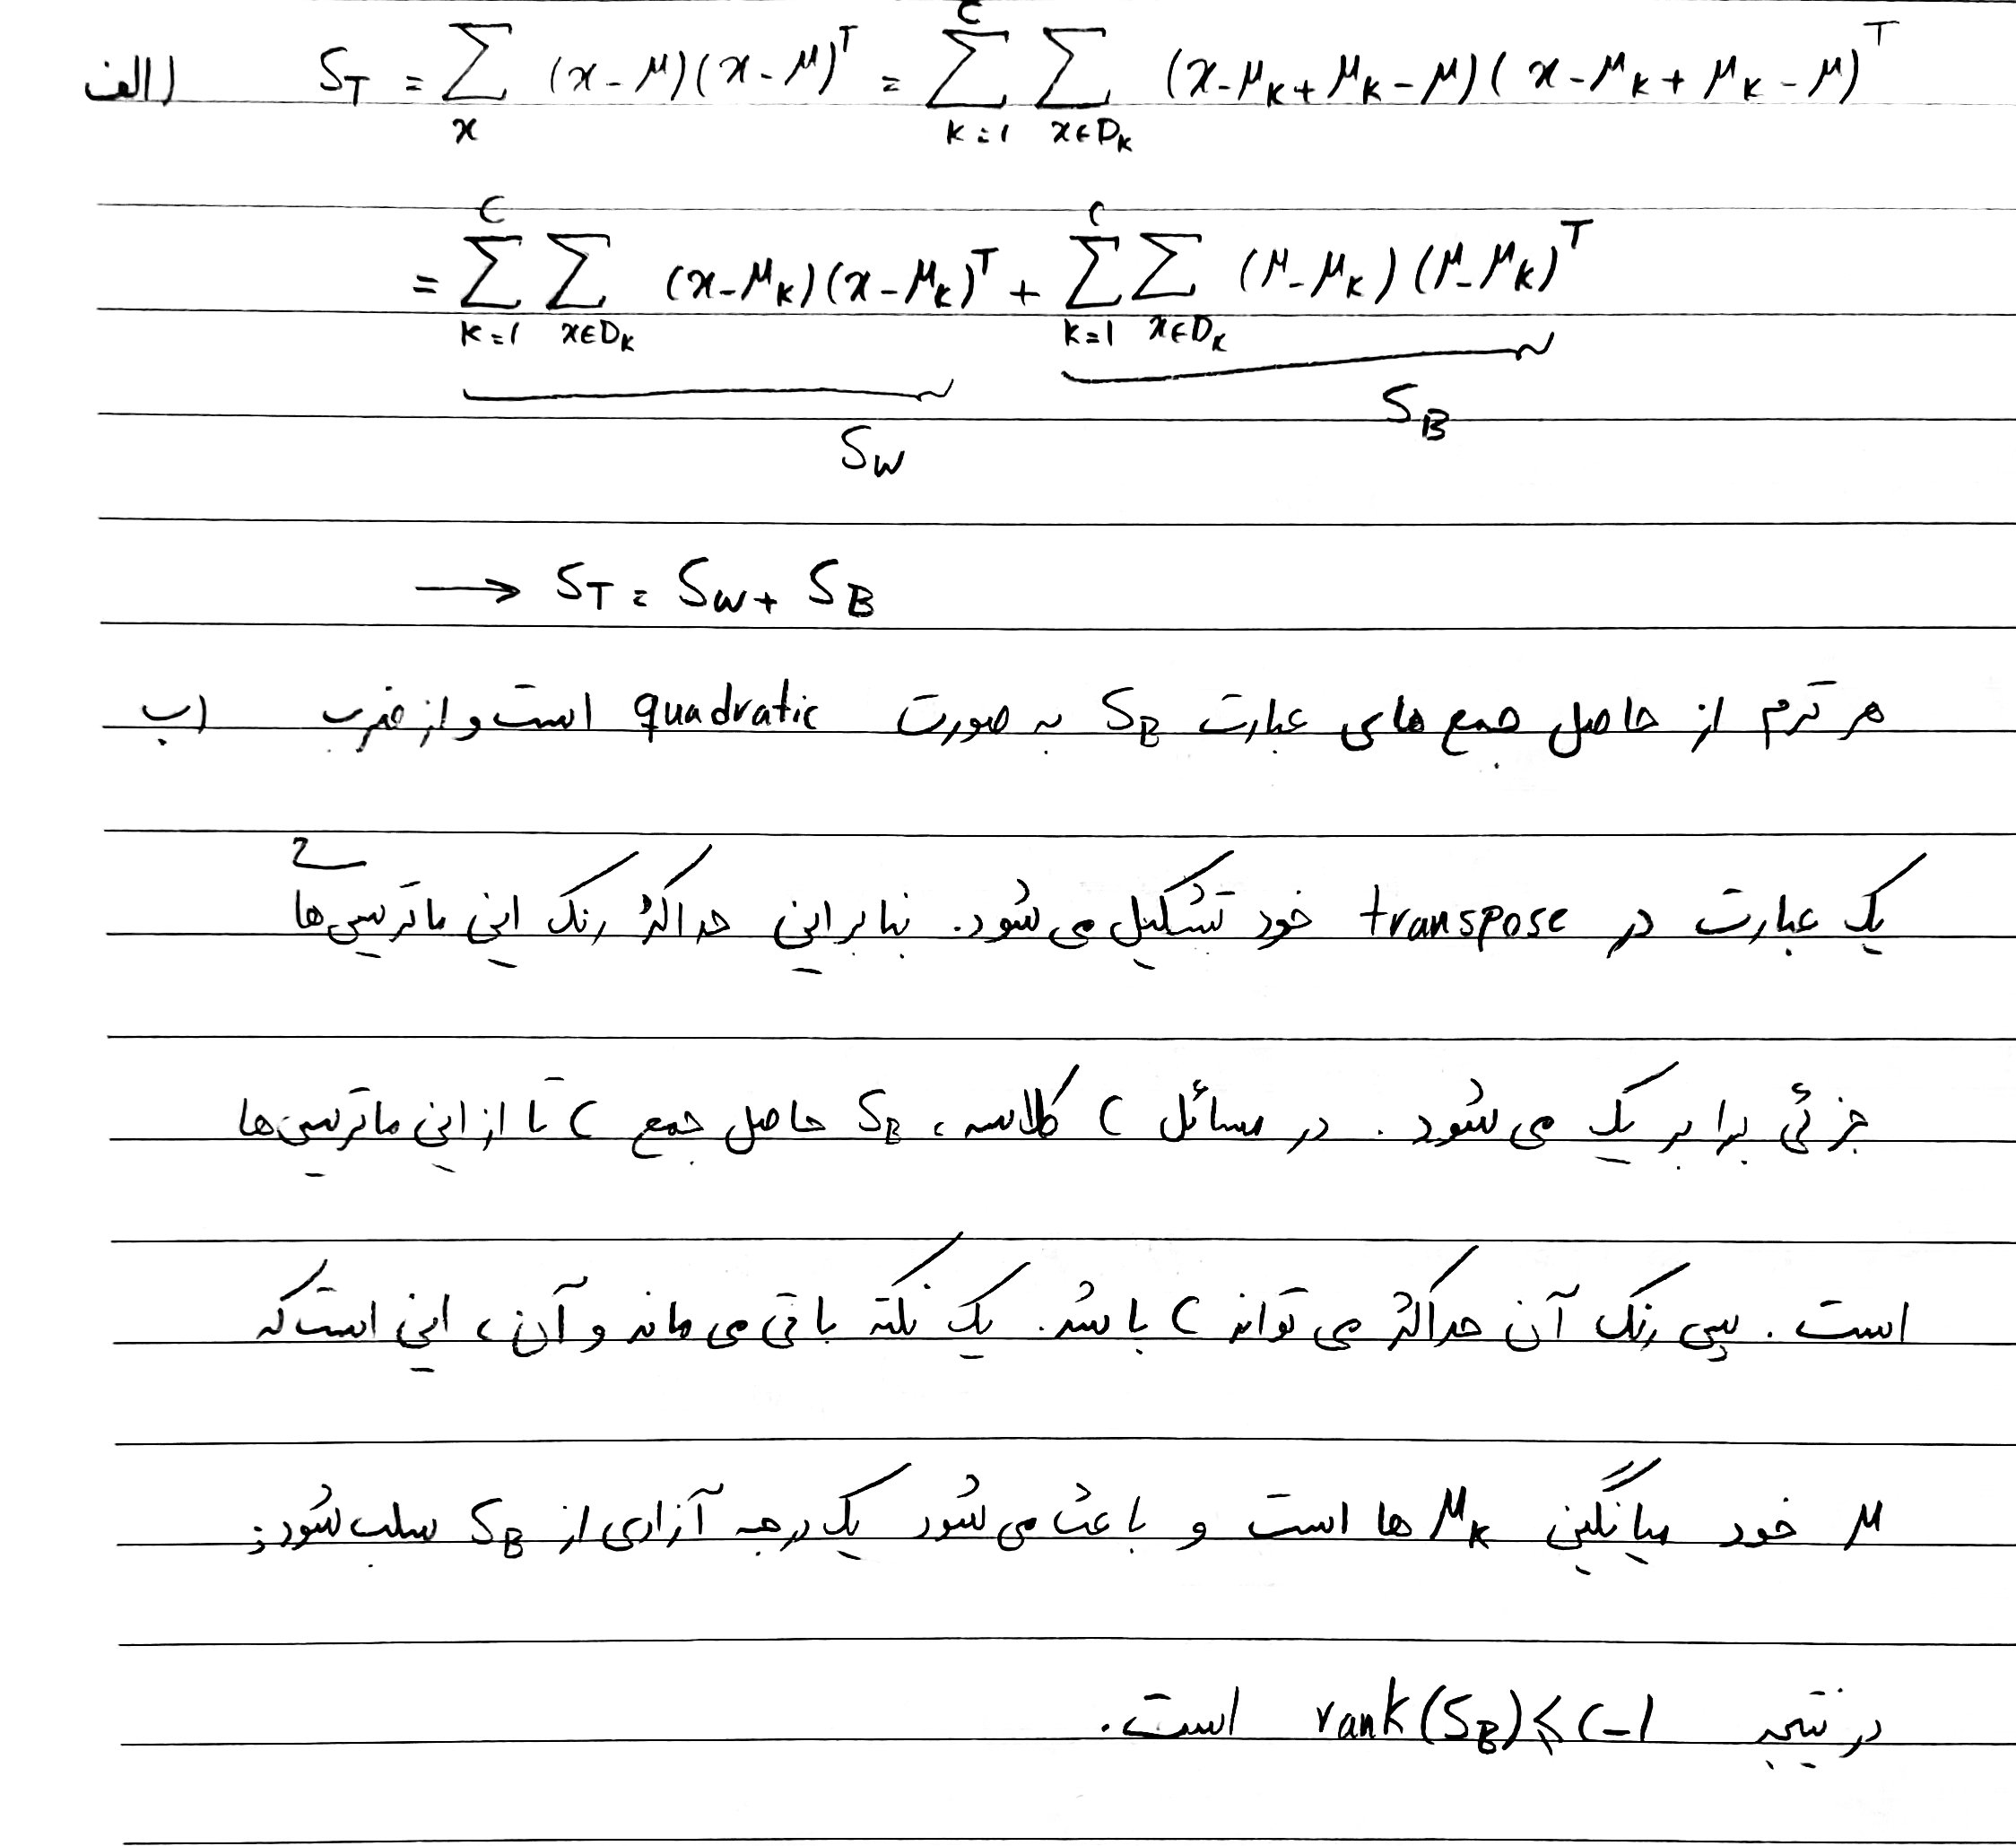
\includegraphics[width=\linewidth]{hand_written/2.jpg}
    \end{center}
\end{figure}

\newpage
\section*{سؤال چهار}
\begin{figure}[h!]
    \begin{center}
    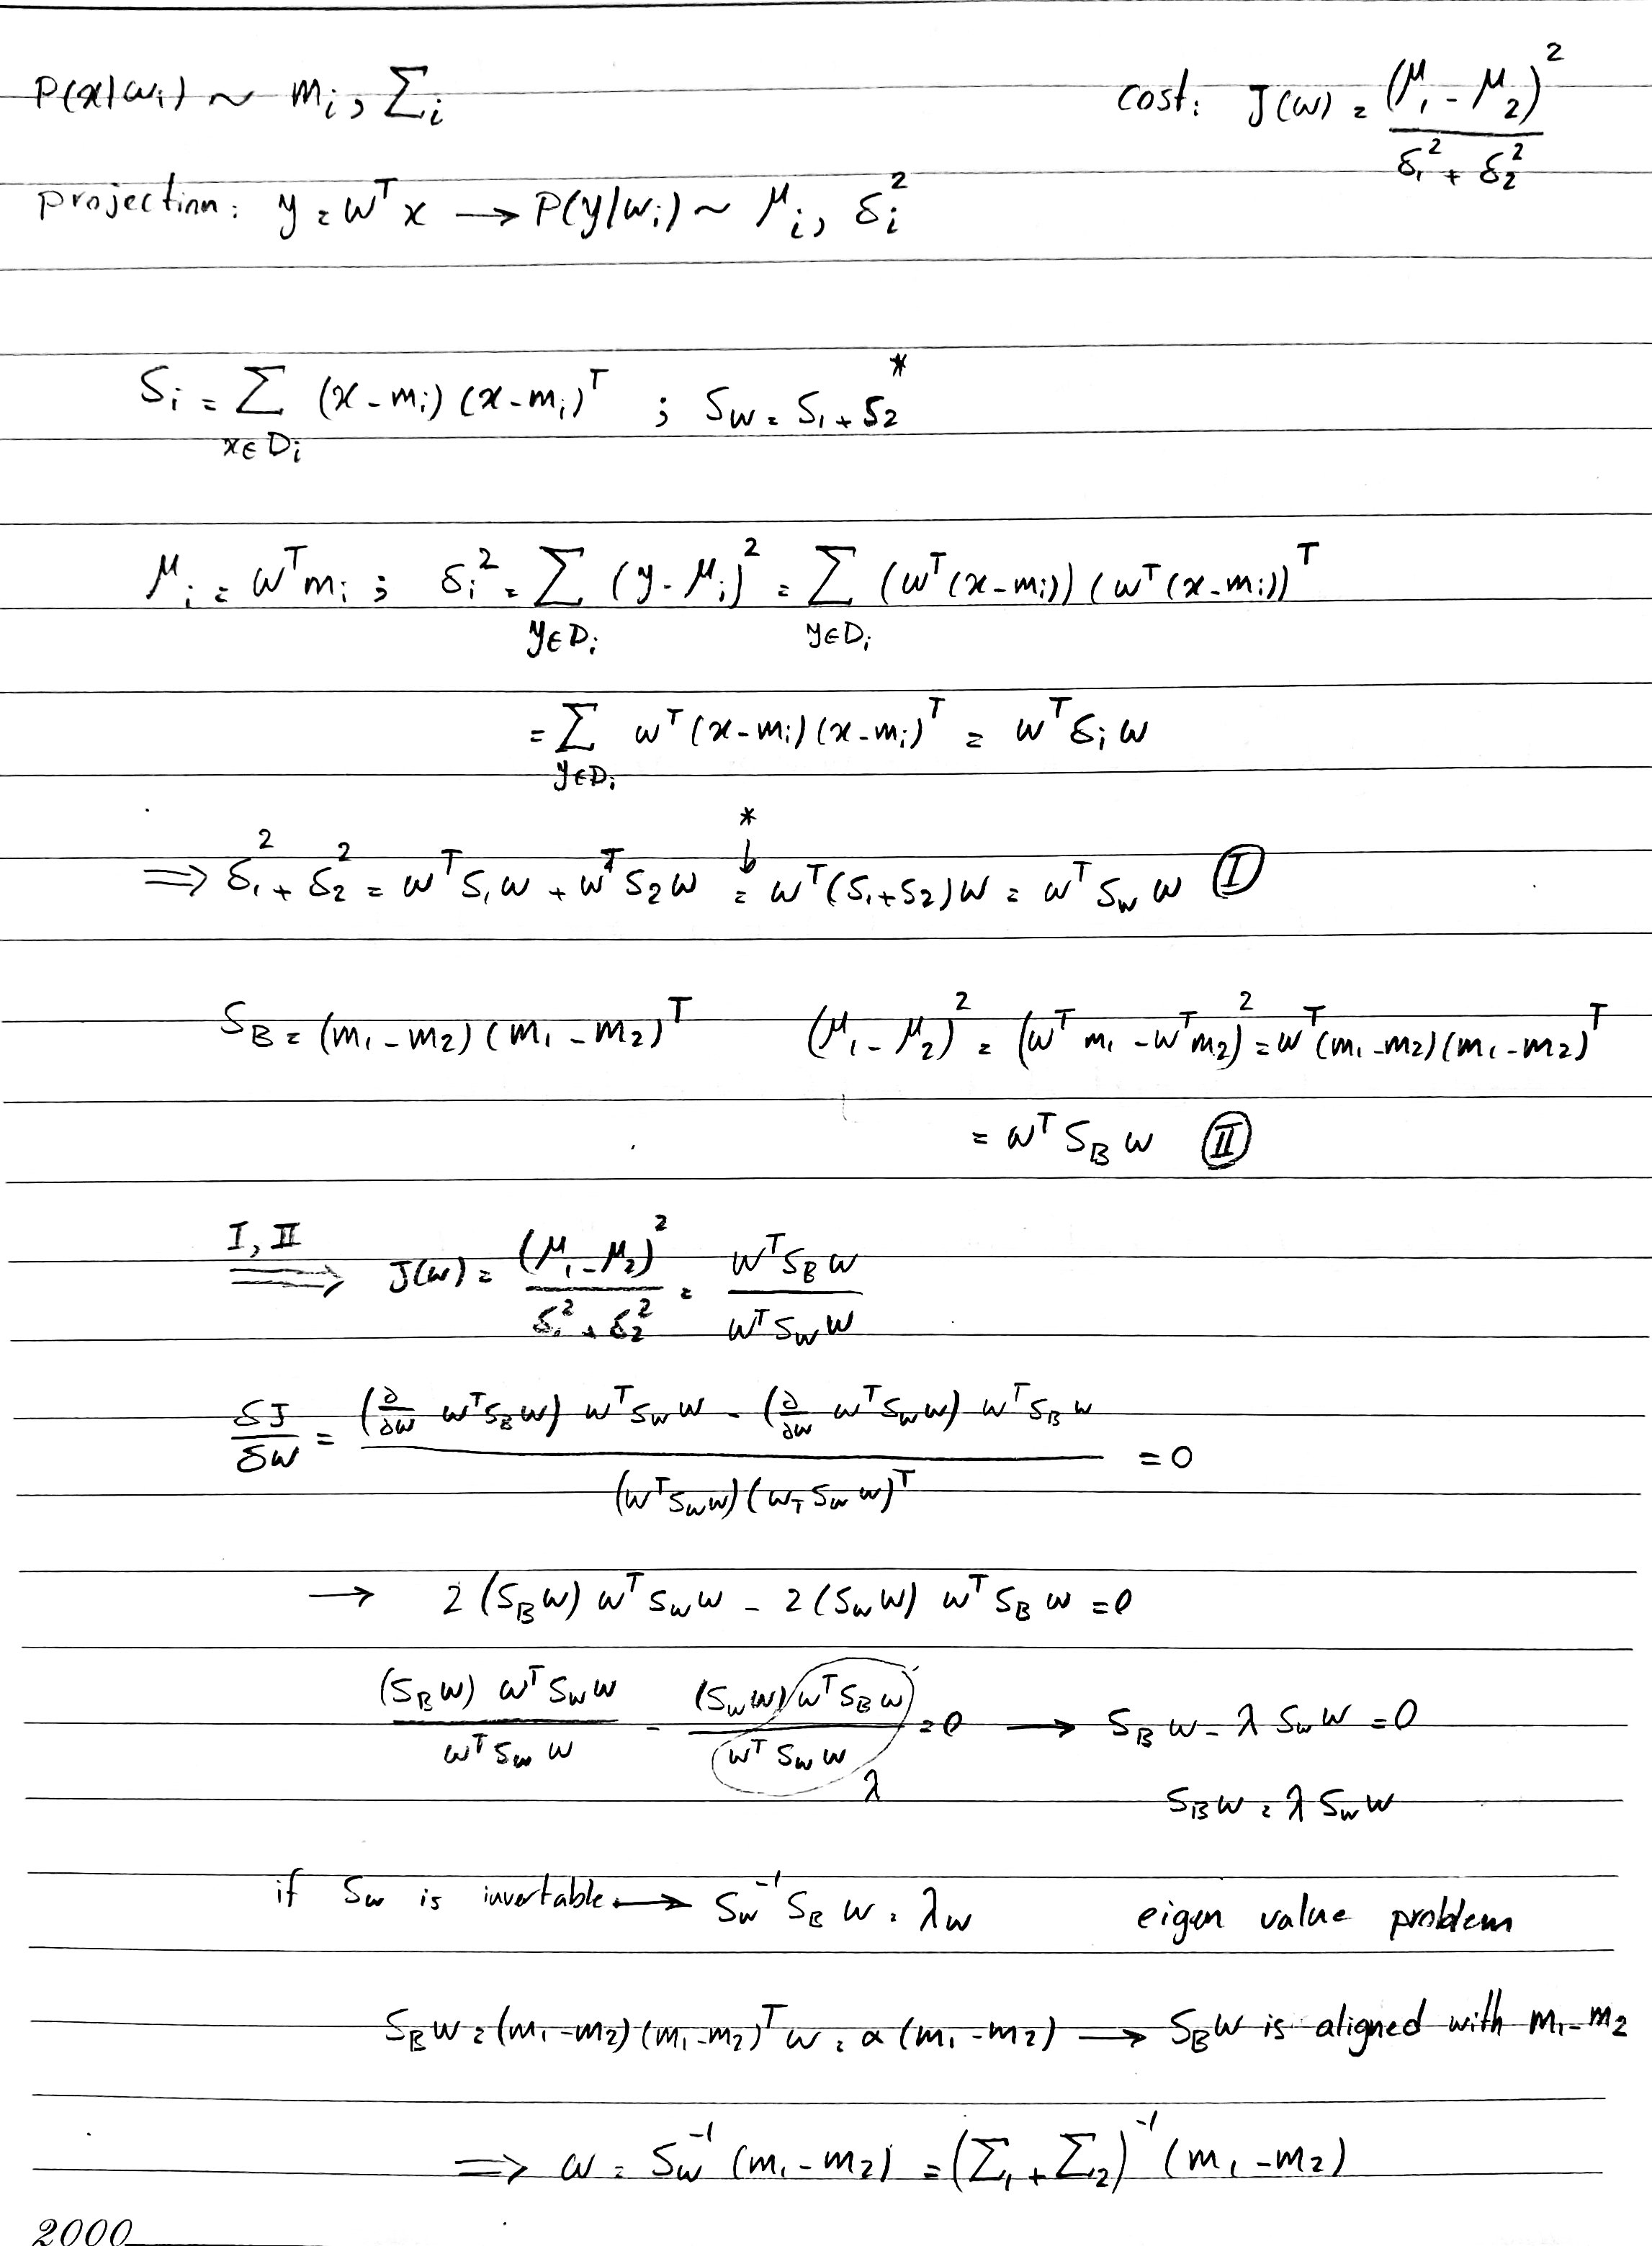
\includegraphics[width=\linewidth]{hand_written/4.jpg}
    \end{center}
\end{figure}

\newpage
\section*{سؤال پنج}
\begin{figure}[h!]
    \begin{center}
    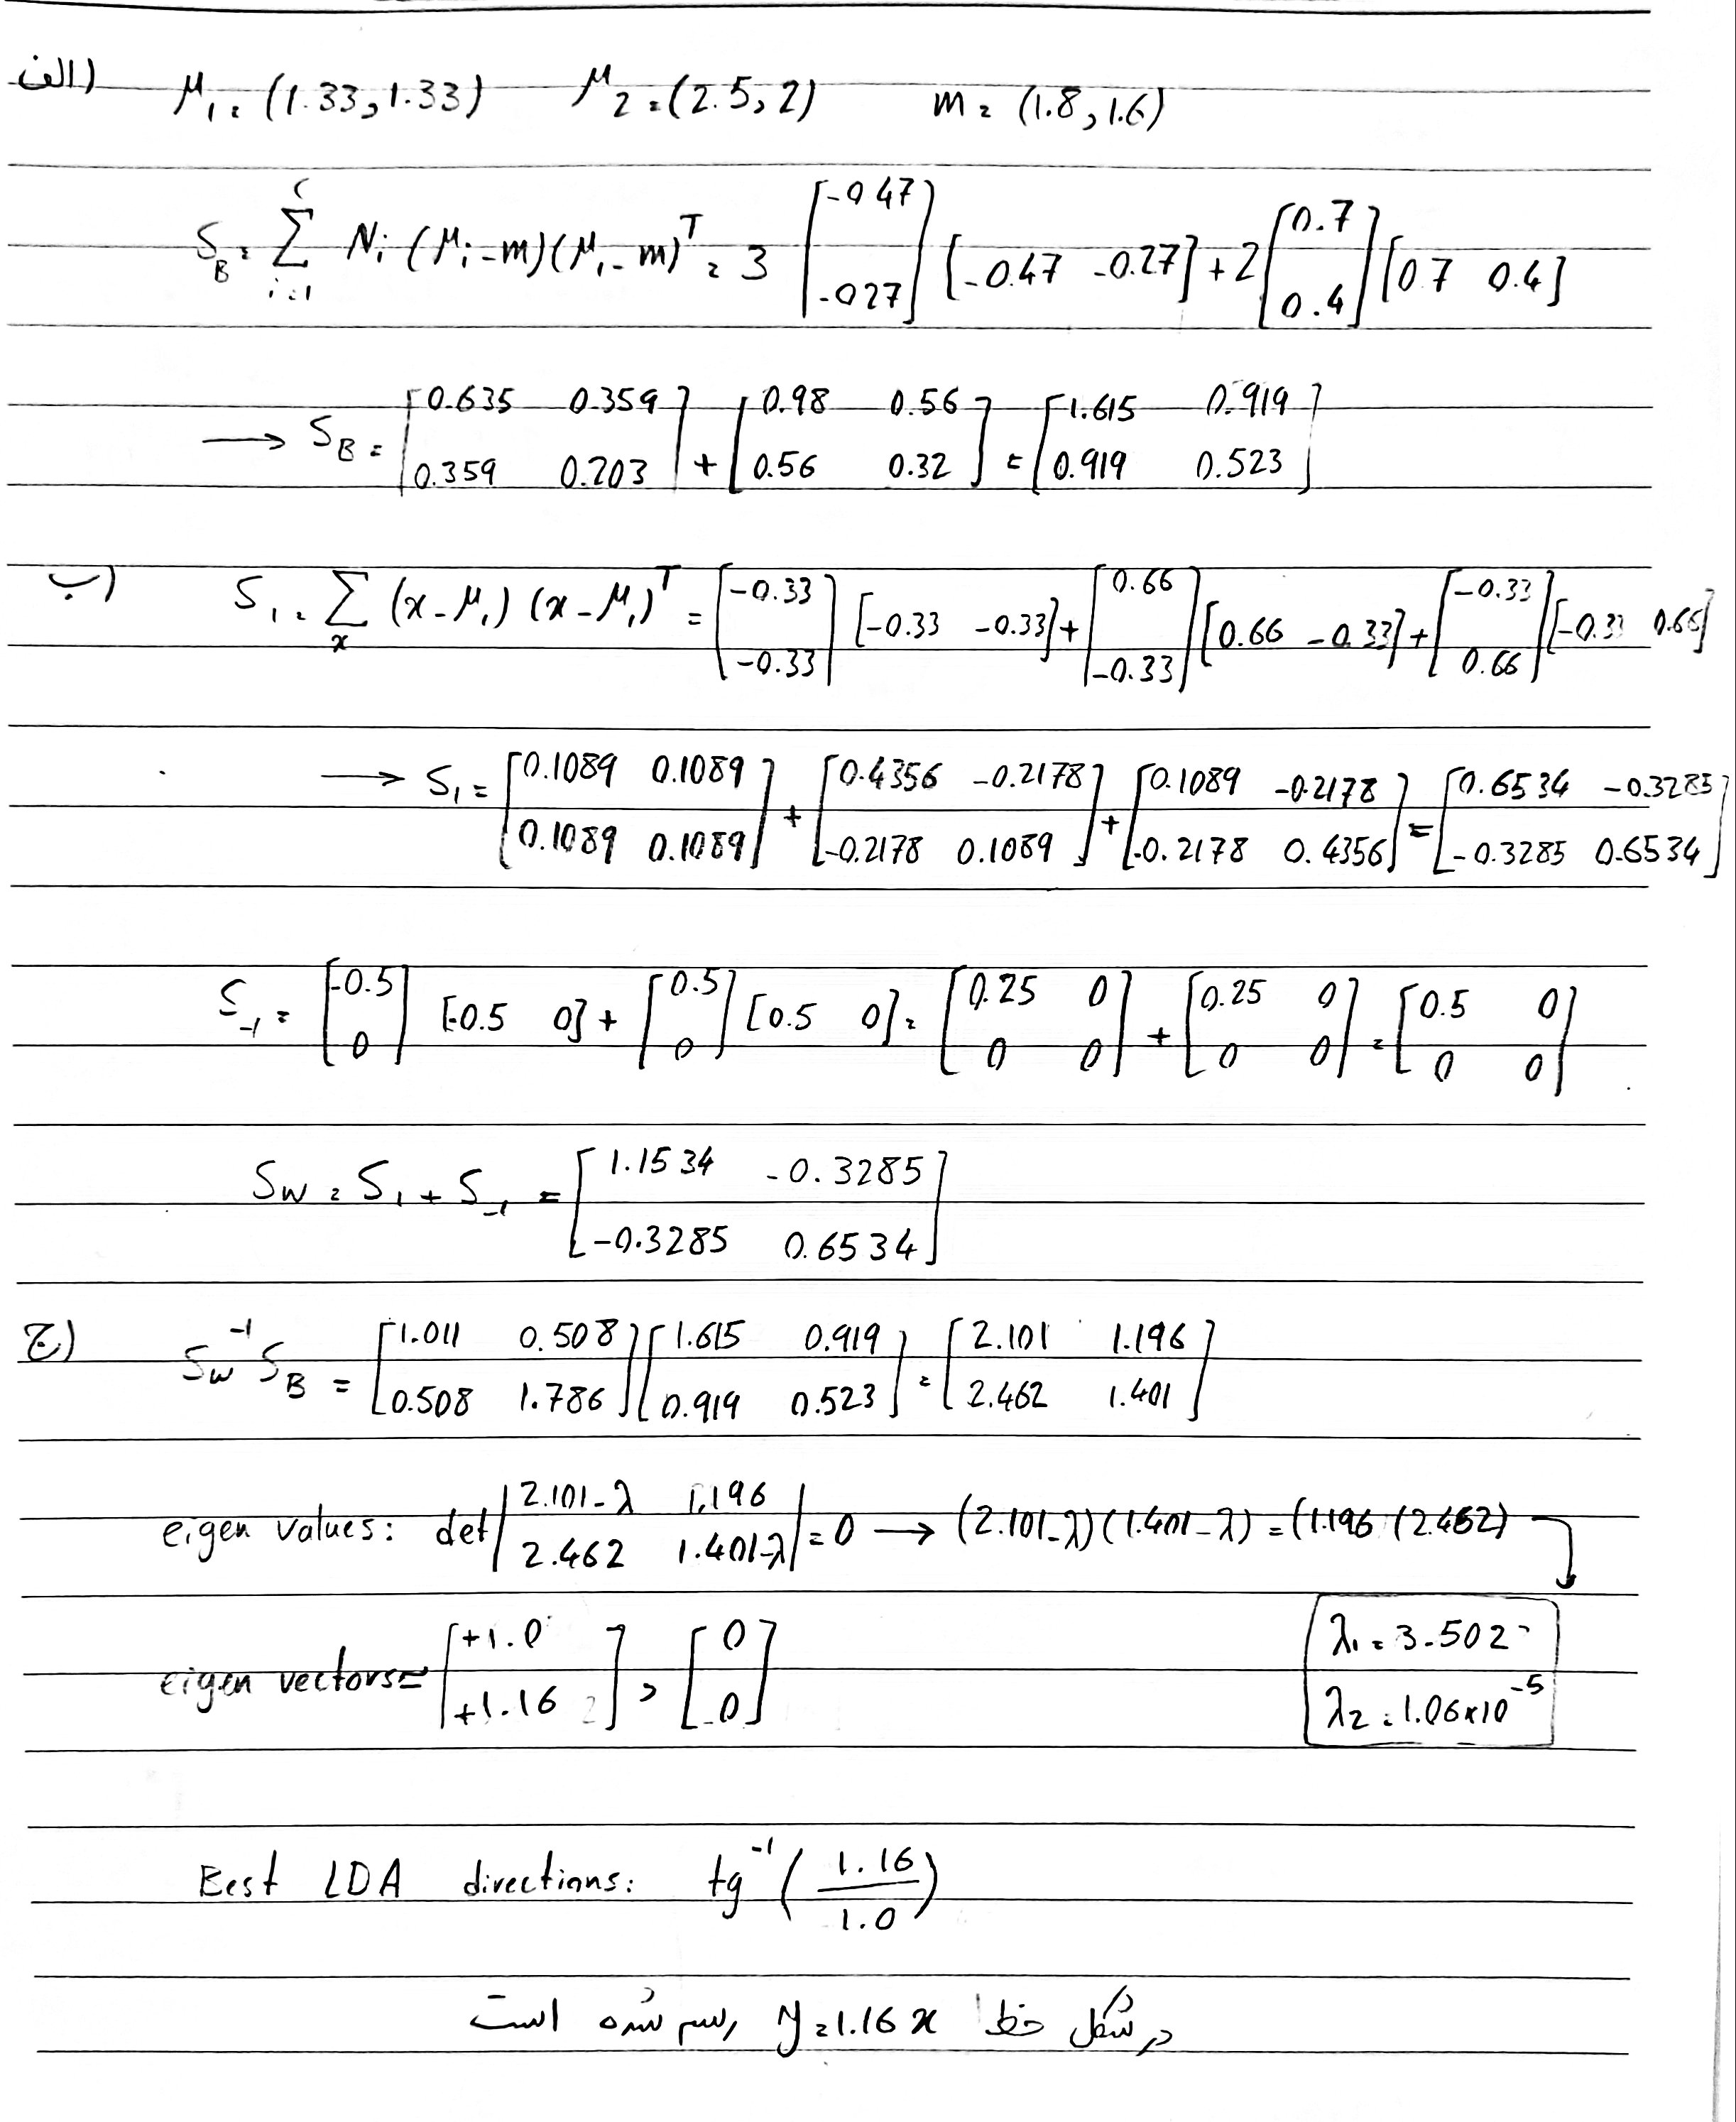
\includegraphics[width=\linewidth]{hand_written/5.jpg}
    \end{center}
\end{figure}
با توجه به شیب خط‌های به دست آمده از قسمت قبل جهت‌های به دست آمده را همراه با داده‌ها رسم می‌کنیم. نقاط قرمز مربوط به $y_{i} = 1$ و نقاط بنفش مربوط به کلاس $y_{i}=-1$ هستند.
\begin{figure}[h!]
    \begin{center}
    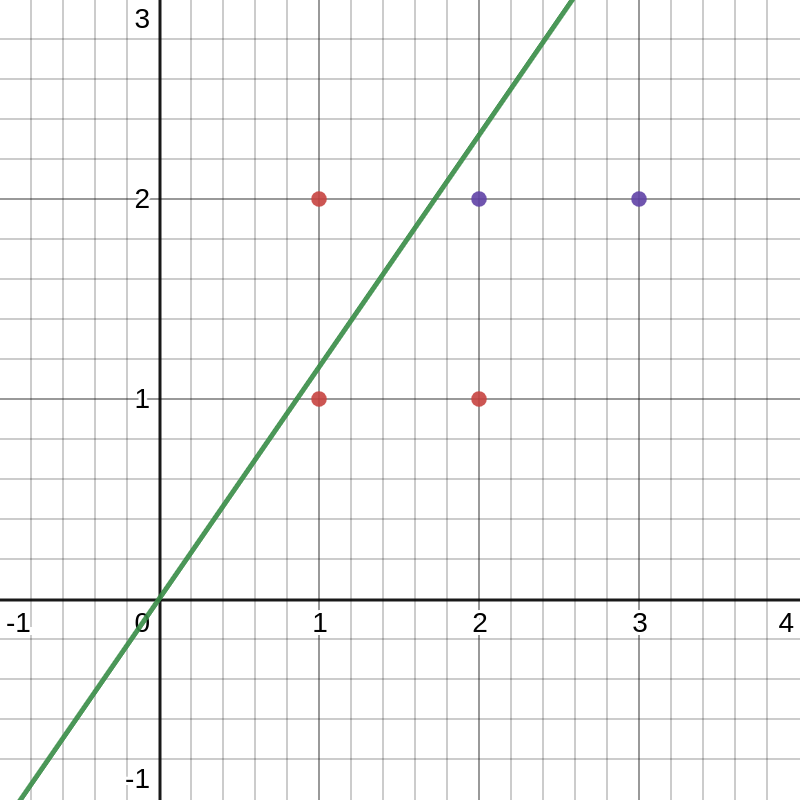
\includegraphics[width=\linewidth]{desmos-graph.png}
    \end{center}
\end{figure}


\newpage
~\newpage
\section*{سؤال شش}
\subsection*{الف}
برای پیاده سازی \lr{SFS} در حلقه \lr{for} بیرونی دو متغیر تعریف می‌کنیم برای یافتن بهترین فیچر جهت اضافه کردن به لیست \lr{selected feature index}. در حلقه \lr{for} درونی که بر روی \lr{i} لوپ می‌زند ابتدا چک می‌کنیم که \lr{i} قبلا انتخاب نشده باشد، سپس بردارهای \lr{x} و \lr{x test} را از روی متغییرهای کلاس و با توجه به ایندکس فیچرهای انتخاب شده تشکیل می‌دهیم و با استفاده از دستورات کتابخانه \lr{scikit learn} دقت آن را بر روی مجموعه تست اندازه گیری می‌کنیم. پس از هر بار ایتریش بر روی متغییر \lr{j} یک ایندکس به زیر مجموعه فیچرها اضافه می‌شود و دقت طبقه بندی آن نیز به لیست \lr{acc list} اضافه می‌شود.
\\
برای رسم نمدار مشابه نمودار مثال از کتابخانه \lr{pandas} و \lr{matplotlib} استفاده شده است. متغییر \lr{th (threshold)} مقداری است که در آن دقت طبقه بندی با زیر مجموعه به دست آمنده بیشتر از ۹۰٪ شود در نمودار با رنگ قرمز رسم شده است. تیک‌های محور \lr{y} نیز لیست بازگردانده شده از متد \lr{forward} می‌باشند. این نمودار در شکل \ref{fig:1} آورده شده است.
\begin{figure}[h!]
    \begin{center}
    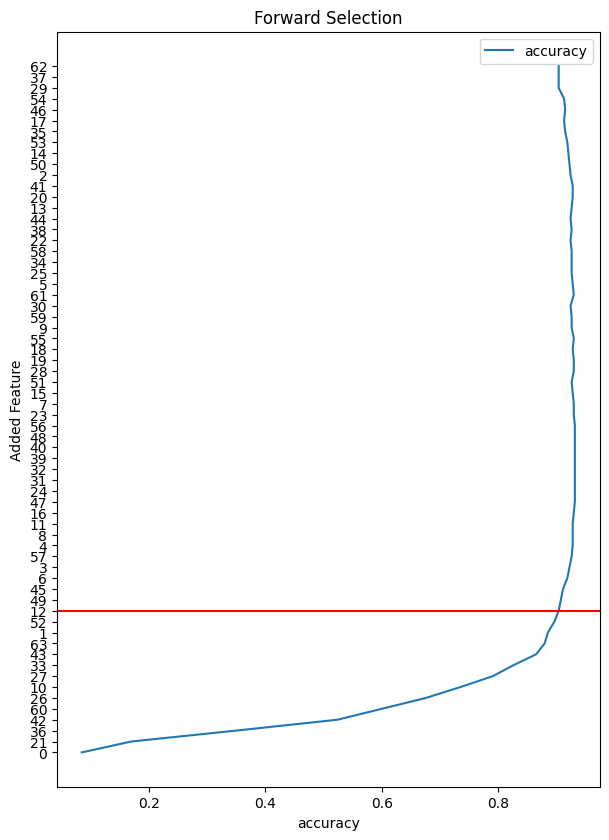
\includegraphics[scale=0.55]{plots/q6_a.png}
    \caption{نتایج اجرای الگوریتم \lr{SFS}}
    \label{fig:1}
    \end{center}
\end{figure}

\subsection*{ب}
این قسمت شباهت زیادی به بخش الف دارد. فقط برای به دست آوردن زیرمجموعه فیچرها از تابع \lr{delete} از کتبخانه \lr{numpy} استفاده می‌کنیم تا بردارهای \lr{x} و \lr{x test} را بسازیم. 
\\
نمودار رسم شده نیز مانند بخش قبل می‌باشد و تنها تفاوت در به دست آوردن مقدار \lr{th} می‌باشد که باید از انتها به ابتدا لوپ زد و مقدار بهینه ترشهولد را به دست آورد. نمودار خواسته شده در شکل \ref{fig:2} نشان داده شده است.
\begin{figure}[h!]
    \begin{center}
    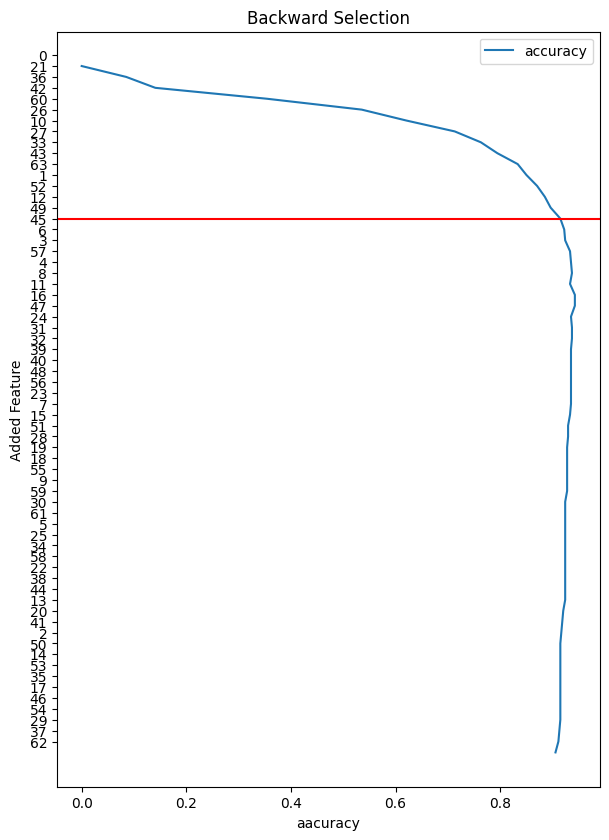
\includegraphics[scale=0.55]{plots/q6_b.png}
    \caption{نتایج اجرای الگوریتم \lr{SBS}}
    \label{fig:2}
    \end{center}
\end{figure}

\newpage
\section*{سؤال هفت}
\subsection*{الف}


\newpage
\section*{سؤال هشت}
\subsection*{الف}


\end{document}